% ----------------------------------------------------------
\chapter{Introdução}
% ----------------------------------------------------------

 O conceito de armadura é tão antigo quanto se possa imaginar. As armaduras tem acompanhado o ser humano através dos tempos. Sempre com o mesmo objetivo final, que é proteger recursos valiosos. Muitas vezes este recurso trata-se da própria vida de quem está sendo protegido pela armadura. Paul Hazell fala em seu livro, Armour Materials, Theory and Design, \cite{Hazell}, sobre o que chama de cebola da sobrevivência. Esta é uma analogia para as varias camadas da proteção, ver figura \ref{fig:0.1}.\\
 
 \begin{figure}[h]
 	\caption{Cebola da sobrevivência destacando a direita as camadas abordadas pelo trabalho.}
 	\centering
 	
\includegraphics{images/cebola_sobrevive}
 	\label{fig:0.1}
 	\fonte{\cite{Hazell} traduzido pelo autor.}
 \end{figure}
O foco deste trabalho é revisar a fundamentação teórica da ferramenta mais usada para estudar a camada 4, não ser penetrado, que é a simulação computacional de impactos balísticos. Há certa interação entre não ser penetrado e não ser adquirido. Inicialmente parece enigmático o conceito de não ser adquirido, porém ele nada mais é do que a habilidade de poder escapar da mira humana ou de qualquer sistema de referenciação do projétil. Sendo assim quando se trata de veículos a velocidade é um dos maiores potencializadores da capacidade de não ser adquirido. \\

Um exemplo para a interação citada anteriormente pode ser dado usando veículos com motores a combustão interna. Os tanques são os veículos militares terrestres mais famosos na cultura popular. Em geral, quando comparados a outros veículos terrestres, os tanques tem o balanço desviado para a camada 4, não ser penetrado. Para cumprir sua função o tanque deve carregar munições e armas que quando somados possuem peso significativamente alto. Além disso é normal que o tanque tenha que assumir uma posição de apoio, logo deve permanecer em uma região específica. Somando as características e funções deste veículo, é natural que se construa um veículo com placas de metal espessas que suportem projeteis de energia cinética considerável. Tal construção gera um desequilíbrio em favor do tanque não ser penetrado, em detrimento dele não ser adquirido.\\ 

\begin{figure}[h]
	\caption{\label{fig:0.2} Veículo M1-Abrams}
	\centering
	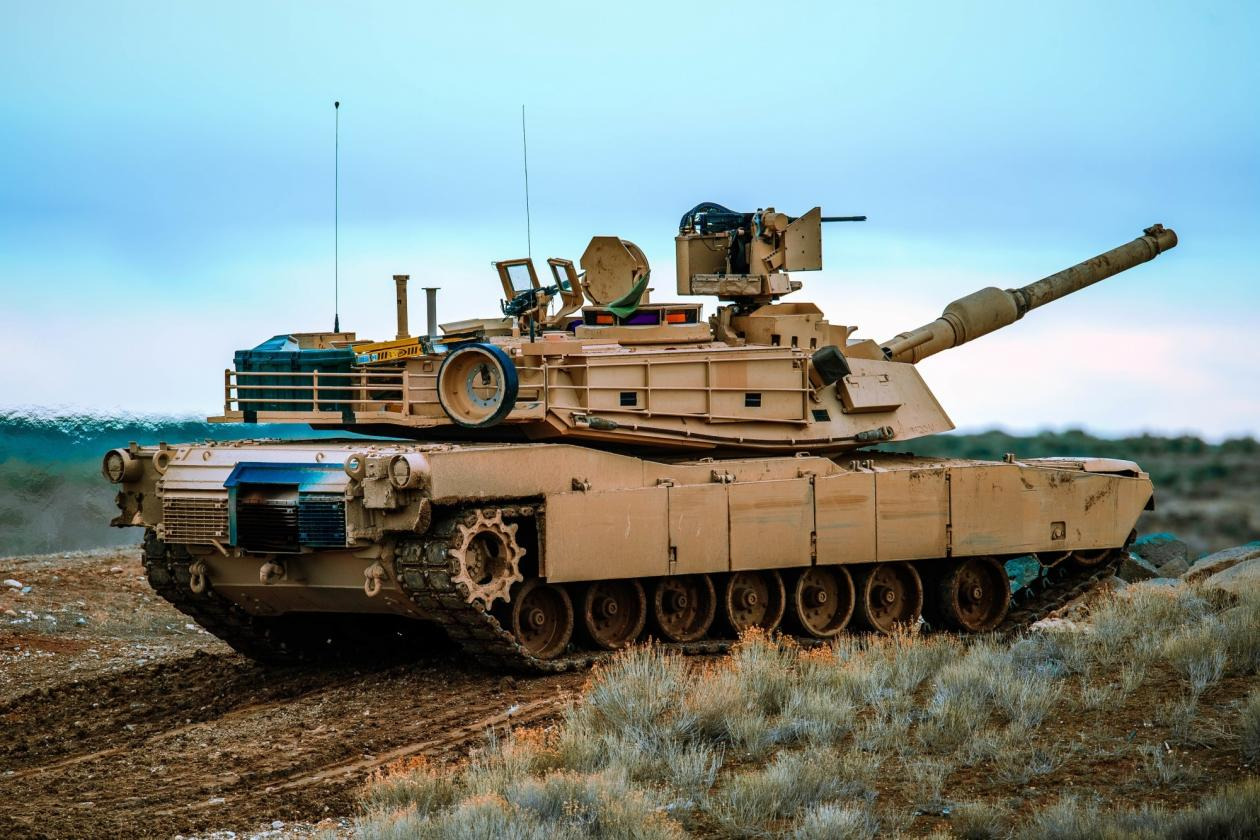
\includegraphics[width=0.7\linewidth]{images/m1-abrams}
	\fonte{https://nationalinterest.org/blog/buzz/us-armys-legendary-m1-abrams-tank-rip-or-ready-war-77621}
\end{figure}

 Do outro lado do espectro estão os veículos mais leves com tarefas variadas. Exemplo disso é o VBMT-LSR do exército brasileiro. Este apresenta desequilíbrio em favor de não ser adquirido, de tal forma que projéteis pesados podem facilmente penetrar sua blindagem. A velocidade e agilidade deste tipo de veículo, tendo um tanque como padrão, aumenta a dificuldade de aquisição. O fato de ter maior dificuldade de aquisição não livra o veículo de ser atingido facilmente por projeteis guiados por sistemas de posicionamento avançados. A motivação da agilidade e rapidez dos veículos leves é o cumprimento de suas funções estratégicas, porém o veículo usa este recurso para sobreviver. \\
 \begin{figure}[h]
 	\caption{\label{fig:0.3} Veículo VBMT-LSR, classificado como veículo leve multitarefa.}
 	\centering
 	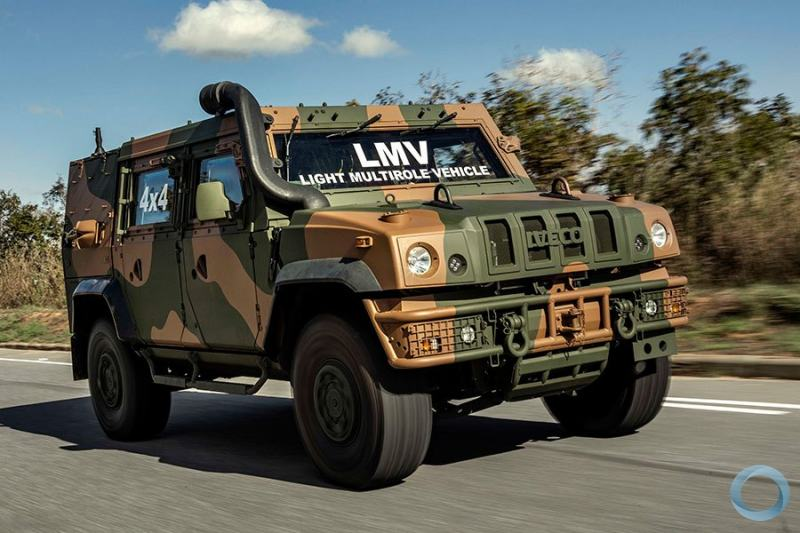
\includegraphics[width=0.7\linewidth]{images/lmv}
 	\fonte{http://www.defesanet.com.br/guarani/noticia/34800/VBMT-LSR---Exercito-Brasileiro-oficializa-a-compra-da-LMV--com-a-IVECO-Veiculos-de-Defesa-/}
 \end{figure} 
\vspace{10mm}

O exemplo mostra o balanço de forma reduzida, dado que existem relações complexas entre as camadas da sobrevivência. Em geral há forte envolvimento da massa do sistema na distribuição de quais camadas são ou não privilegiadas. Normalmente o aumento da capacidade de absorver impacto se dá por meio da inserção de placas massivas, diminuindo a mobilidade do sistema. Este trabalho tem foco na fundamentação da simulação de impacto balístico em veículos leves e coletes pessoais, portanto apenas projeteis pequenos com velocidade abaixo de $ 2000 m/s$ estão contemplados. \\

Para desenvolver este tipo de proteção é necessário entender como ela se comportará face aos impactos que irá sofrer. É possível fazer todo o estudo de comportamento e de possíveis melhorias usando apenas experimentação, porém esta não é a melhor opção em relação aos valores investidos. Um caminho viável para tal é usar simulações computacionais aliadas à experimentação. Este trabalho apresenta a fundamentação de uma ferramenta específica, a simulação computacional, aplicada em um contexto particular, que é o impacto projéteis consideravelmente pequenos em baixa velocidade. \\

As bases teóricas para a simulação computacional de um evento balístico são o foco desta revisão. A figura \ref{fig:diagramalog} mostra um diagrama com todos os maiores elementos da fundamentação teórica de uma simulação computacional de um impacto balístico. Nesta figura os retângulos são áreas abrangentes, enquanto os hexágonos são tópicos específicos da sua respectiva área abrangente. Cada área e seus tópicos serão revisados no trabalho, porém cabe aqui uma pequena introdução com intuito mostrar o posicionamento de cada área e a respectiva motivação de abordar tal assunto. \\

A contribuição da mecânica do contínuo é a definição das deformações finitesimais e das leis básicas do equilíbrio termodinâmico. Em um impacto balístico o projetil penetra o anteparo, gerando grandes deslocamentos e por conseguinte deformações. A deformação é um dado de entrada no modelo constitutivo, portanto descrever corretamente o tipo de deformação é muito importante em um evento balístico. O diagrama da figura \ref{fig:diagramalog} não mostra esta inserção para manter sua simplicidade e linearidade. Mesmo não estando evidente no diagrama a definição das deformações finitesimais é importante, já que este é um ponto de divergência entre o tipo de simulação mais comum na indústria, que usa deformações infinitesimais, e o tipo usado para simular um evento balístico. Sendo assim o primeiro passo dado no capítulo que aborda a mecânica do contínuo é a definição das deformações finitesimais. Os princípios termodinâmicos básicos limitam as possíveis configurações termodinâmicas da solução. A equação diferencial resolvida pelo método dos elementos finitos advém de um destes princípios, que é o balanço de momento linear. Portanto a definição dos princípios termodinâmicos básicos é a segunda etapa do capítulo que trata a mecânica do contínuo. \\

O método dos elementos finitos é abordado depois da mecânica do contínuo por ser usado para resolver o balanço de momento linear. A consideração de todos os fatores envolvidos em uma simulação de impacto balístico leva a um problema de alta complexidade, portanto não é interessante apresentar a fundamentação da ferramenta neste ambiente. A apresentação feita neste trabalho usa um problema simplificado, pois o objetivo é mostrar os constituintes básicos que por sua vez estão presentes desde o mais simples até o mais complexo dos problemas. \\

O comportamento dos materiais quando impactados é fundamentado pela plasticidade computacional, portanto este assunto é brevemente abordado para a posterior exposição dos modelos constitutivos mais usados na aplicação balística. O modelo constitutivo é acoplado ao método dos elementos finitos e é responsável por calcular o estado de tensão a depender de variáveis termodinâmicas da solução em um certo ponto e momento do tempo. Basicamente ele recebe variáveis termodinâmicas e devolve tensões, que por sua vez são usadas para resolver o equilíbrio mecânico, gerando um processo iterativo de resolução. \\

Por fim a mecânica da penetração é usada para definir o problema resolvido, por meio da geometria e das condições de contorno. Além disso a interpretação da simulação é feita com base nas teorias deste campo, por conseguinte é importante para um analista saber quais são, em teoria, os resultados possíveis da simulação. A mecânica do da penetração é um vasto campo, sendo assim o trabalho aborda a fundamentação teórica dos impactos em estruturas leves, com enfoque particular nos materiais cerâmicos. 

\begin{figure}[H]
 	\caption{\label{fig:diagramalog} Diagrama lógico da fundamentação teórica de uma simulação computacional de um impacto balístico}
 	\centering
 	\includegraphics[width=0.8\linewidth]{images/Diagrama Lógico TCC.png}
 	\fonte{O autor 2020}
 \end{figure} 
 


% ----------------------------------------------------------
\section{Objetivos}
% ----------------------------------------------------------

% ----------------------------------------------------------
\subsection{Objetivo Geral}
% ----------------------------------------------------------

Revisar a fundamentação teórica das áreas de maior influência na simulação computacional de um evento de impacto balístico.

% ----------------------------------------------------------
\subsection{Objetivos Específicos}
% ----------------------------------------------------------

\begin{itemize}
    \item Revisar os fundamentos da mecânica do contínuo com foco na descrição de deformações finitesimais e nas leis de equilíbrio.
    \item Revisar os fundamentos do método dos elementos finitos com foco em sistemas dinâmicos.
    \item Revisar os fundamentos da plasticidade computacional e apresentar os modelos constitutivos mais usados quando altas taxas de deformação estão presentes.
    \item Revisar o processo de penetração de projéteis com velocidades inferiores a $2000 m/s$, com enfoque em alvos feitos de material cerâmico.
\end{itemize}